\documentclass[10pt]{article}
\usepackage[final]{graphicx}
\usepackage{amsfonts}
\usepackage{float}
\usepackage{amsmath}
\usepackage{ dsfont }
% Take out later when you remove highlights
\usepackage{soul}

\topmargin-.5in
\textwidth6.6in
\textheight9in
\oddsidemargin0in

\def\ds{\displaystyle}
\def\d{\partial}

\begin{document}

\centerline{\large \bf Identifying Precision Treatment for Rheumatoid Arthritis with Reinforcement Learning}

\vspace{.1truein}

\def\thefootnote{\arabic{footnote}}
\begin{center}
  Chixiang Chen\footnote{Biostatistics, Pennsylvania State University},
  Ashley Gannon\footnote{Scientific Computing, Florida State University},
  Duwani Katumullage\footnote{Statistics, Sam Houston State University},
  Miaoqi Li\footnote{Mathematical Sciences, University of Cincinnati},
  Mengfei Liu\footnote{Statistics, George Washington University},
  Rebecca North\footnote{Statistics, NC State University},
  Jialu Wang\footnote{Statistics, College of William and Mary}
\end{center}

%\vspace{.1truein}

\begin{center}
Faculty Mentors: Grant Weller, Victoria Mansfield, Yingong Guo\footnote{Savvysherpa},
Daniel Luckett \footnote{UNC}
\end{center}

\vspace{.3truein}
\centerline{\bf Abstract}

Rheumatoid Arthritis (RA) is an autoimmune disease that causes chronic inflammation in the lining of joints leading to multiple complications including painful swelling, long-term damage from bone erosion, and joint deformity. Diagnosing and treating patients with RA is challenging due to several factors: there is a high rate of comorbid conditions that effect various organs, there aren't clinically validated methods for measuring disease progression, and an optimal treatment regime has not been identified. In this work, we examine the empirical treatment regimes of over 6,500 RA patients to propose a framework with the ability to identify an optimal dynamic treatment regime (DTR). 

\begin{itemize}
\item Summarize the results presented in the report, and the contributions
of your research.

\item Readers should not have to look at the rest of the paper in order to 
understand the abstract.

\item Keep it short and to the point.
\end{itemize}

\section{Introduction}

Rheumatoid arthritis (RA) is a heterogeneous, chronic inflammatory disease that affects 1\% of people worldwide (Cite 1 and 2 from abstract). RA predominately effects the lining of joints causing pain and inflammatory flare ups. It also effects organs such as the heart, skin, eyes and lungs causing growths, vasculitis, scleritis, Sjogren's syndrome and a laundry list of other ailments. In addition to the discomfort and co-morbid conditions, patients diagnosed with RA have a 60\% increase in the risk of heart attack one year after diagnosis and are twice as likely as the average person to develop depression. (CITE 3 from abstract) The variety of symptoms presented in a patient with RA makes it a difficult disease to diagnose and manage. Additionally, there is currently no single, autoantibody specific diagnostic test available to diagnose patients (CITE 4 from abstract) and the American College of Rheumatology (ACR) does not provide an optimal treatment regime to follow once the patient has been diagnosed. Thus, determining which of the many treatment regimes provided by the ACR is the optimal treatment regime for RA is the focus of this work.

Because RA is a chronic illness, it is imperative to develop a long-term treatment strategy. Treatments vary from person to person and can depend on factors such as treatment history, disease state, age, personal preferences, etc.. Dynamic treatment regimes (DTRs) have been used to generate long-term individualized treatment plans for patients with chronic illnesses (cite 8). In theory, this framework maps an individual's input variables to an optimized set of possible treatment decisions. In reality, it is an onerous task to identify optimal DTRs from large data sets. One possible way to approximate DTRs is to use a machine learning approach, specifically a reinforcement learning approach. Reinforcement learning can be used to maximize the expected outcome and produce a data-driven policy. In this work, we will implement a Q-learning algorithm, a reinforcement learning approach, in an attempt to identify an optimal treatment regime for RA patients based off of their input variables.

Q-learning has become a popular method used to identify optimal DTRs from observational studies,(CITE 9 10 and 11) and is an appropriate method to apply to the provided data set. The original dataset in this work is composed of longitudinal data derived from observational medical and prescription medication claims of over 6,500 RA patients. Most studies using Q-learning to identify DTRs assume that data is collected at small, finite numbers of treatment intervals. In this data set, there exists at minimum 1 year of claims following diagnosis and a minimum of 6 months of claims data prior to diagnosis for each patient. All patient attributes in this data set are updated on a weekly basis. Applying a Q-learning algorithm to this dataset can be challenging due to an imbalance of observation in treatments, potential latent confounds, and unclear implementation instructions for treatment intervals. Our team will address how we handled these difficulties in the approach section.

In this work, we perform descriptive statistics on the orginal data set and use these observations to collapse the data set to monthly observations. On the new monthly data set, we implement a general linearized model (GLM) on our first two months and a Q-learning algorithm on a three month period. While there are several studies aiming to identify the comparative effectiveness of DTR for RA patients, to our knowledge a data-driven effort to identify an optimal DTR for RA has not been published.  

\section{Data Processing}

\subsection{Descriptive Statistics}
To better understand the initial data set provided, we perform descriptive statistical analyses on the attributes presented for each patient. These attributes include categories such as age, gender, medical appointments, specific treatments, and comorbidity conditions. This is an important step in this work as it will help us justify models we develop later on. 

The first attributes we look at are gender age and comorbidities. From Table \ref{tab: age_gender_comorbid_full}, we note that 74\% of the population is female and between the ages of 37 to 57. Since nearly three times as many women are diagnosed with RA than men and RA most commonly develops between the ages of 30 and 60, our dataset does a fair job representing the general population of people diagnosed with RA. We can also note that there are several comorbidities listed that are not common within the given population (<5\%).  The top two most common comorbidities are hypertension and COPD. 

\begin{table}[H]
%	\centering
	\begin{tabular}{l|l|l|l}
		\hline
		~ & member (N = 6846) & ~ & member (N = 6846)\\
		\hline
		\bf{Age at First Diagnosis} & ~ & \bf{Dementia} & ~\\
		\hline
		min & 12 & Prior & 7 (0)\\
		\hline
		max & 64 & Post & 11 (0)\\
		\hline
		mean (standard deviation) & 47.26 $\pm$ 10.99 & \bf{Diabetes} & ~\\
		\hline
		median (interquartile range) & 50.00 (41.00, 56.00) & Prior & 782 (11)\\
		\hline
		\bf{Gender} & ~ & Post & 866 (13)\\
		\hline
		Male & 1,753 (26) & \bf{Hypertension} & ~\\
		\hline
		Female & 5,093 (74) & Prior & 2182 (32) \\
		\hline
		\bf{AIDS/HIV} & ~ & Post & 2315 (34)\\
		\hline
		Prior & 9 (0) & \bf{Liver Disease} & ~\\
		\hline
		Post & 13 (0) & Prior & 433 (6)\\
		\hline
		\bf{Acute Myocardial Infarction} & ~ & Post & 557 (8)\\
		\hline
		Prior & 67 (1) & \bf{Paralysis} & ~\\
		\hline
		Post & 81 (1) & Prior & 34 (0)\\
		\hline
		\bf{Angina} & ~ & Post & 32 (0)\\
		\hline
		Prior & 409 (6) & \bf{Peripheral Vascular Disease} & ~\\
		\hline
		Post & 417 (6) & Prior & 243 (4)\\
		\hline
		\bf{Cancer} & ~ & Post & 275 (4)\\
		\hline
		Prior & 294 (4) & \bf{Renal Failure} & ~\\
		\hline
		Post & 357 (5) & Prior & 90 (1)\\
		\hline
		\bf{Cerebrovascular Disease} & ~ & Post & 192 (3)\\
		\hline
		Prior & 303 (4) & \bf{Ulcers} & ~\\
		\hline
		Post & 296 (4) & Prior & 119 (2)\\
		\hline
		\bf{Congestive Heart Failure} & ~ & Post & 97 (1)\\
		\hline
		Prior & 131 (2) & \bf{Depression} & ~\\
		\hline
		Post & 192 (3) & Prior & 1,276 (19)\\
		\hline
		\bf{COPD} & ~ & Post & 1,129 (16)\\
		\hline
		Prior & 1,423 (21) & \bf{Skin Ulcers} & ~\\
		\hline
		Post & 1,296 (19) & Prior & 865 (13)\\
		\hline
		~ & ~ & Post & 565 (8) \\
		\hline
	\end{tabular}
	\caption{Descriptive Table of Age, Gender and Comorbidities. Continuous data is summarized using a minimum, maximum, mean, and median. The mean includes a standard deviation. The median includes the upper and lower quartiles. The remaining binary data is summarized by their frequency and by the percent of the population with the comorbidity (values in ())}
	\label{tab: age_gender_comorbid_full}
\end{table}

\begin{table}[H]
	\centering
	\begin{tabular}{l|l|l|l|l}
		\textbf{Flag Number} & \textbf{DMARD} & \textbf{NSAID} & \textbf{Glucocorticoid} & \textbf{Opioid} \\
		\hline
		0 & 2,699,454 & 3,057,015 & 3,063,331 & 3,183,441 \\
		\hline
		1 & 499,371 & 141,810 & 135,494 & 15,384 \\
		\hline
		\textbf{Percent of population:} & 15.61\% & 4.43\% & 4.24\% & 0.48\% \\
		\hline
	\end{tabular}
	\caption{Descriptive table of the amount of times a medication is prescribed for the entire dataset}
	\label{tab:prescription_rates}
\end{table}

We also need to know if all patients in this dataset receive treatment for their illness. From Table \ref{tab:prescription_rates} we see that it is more common for an RA patient in this dataset to not seek treatment for their illness. We can also note that of the prescribed medications, the most commonly prescribed are Disease-modifying antirheumatic drugs (DMARDs), nonsteroidal Anti-inflammatory Drugs (NSAIDs) and glucocorticoids being prescibed at roughly the same frequencies and opioids prescribed the least. 
 
Figure \ref{fig:PrescriptionFrequency} is created to represent the population of patients who were treated for RA. Here we observe the most frequently prescribed medications for each group of treatments: DMARDs, NSAIDs, glucocorticoids, and opioids. We find that the most frequently prescribed DMARD is Methotrexate sodium, 36\% of the time that a DMARD is prescribed, the most frequently prescribed NSAID is Celecoxib, 30\% of the time an NSAID is prescribed, the most frequently prescribed glucocorticoid is Prednisone, 97\% of the time a glucocorticoid is prescribed, and finally the most frequently prescribed opioid is Oxycodone HCL, 47\% of the time an opioid is prescribed.  

\begin{figure}[H]
	\centering
	%\captionsetup{justification=centering}
	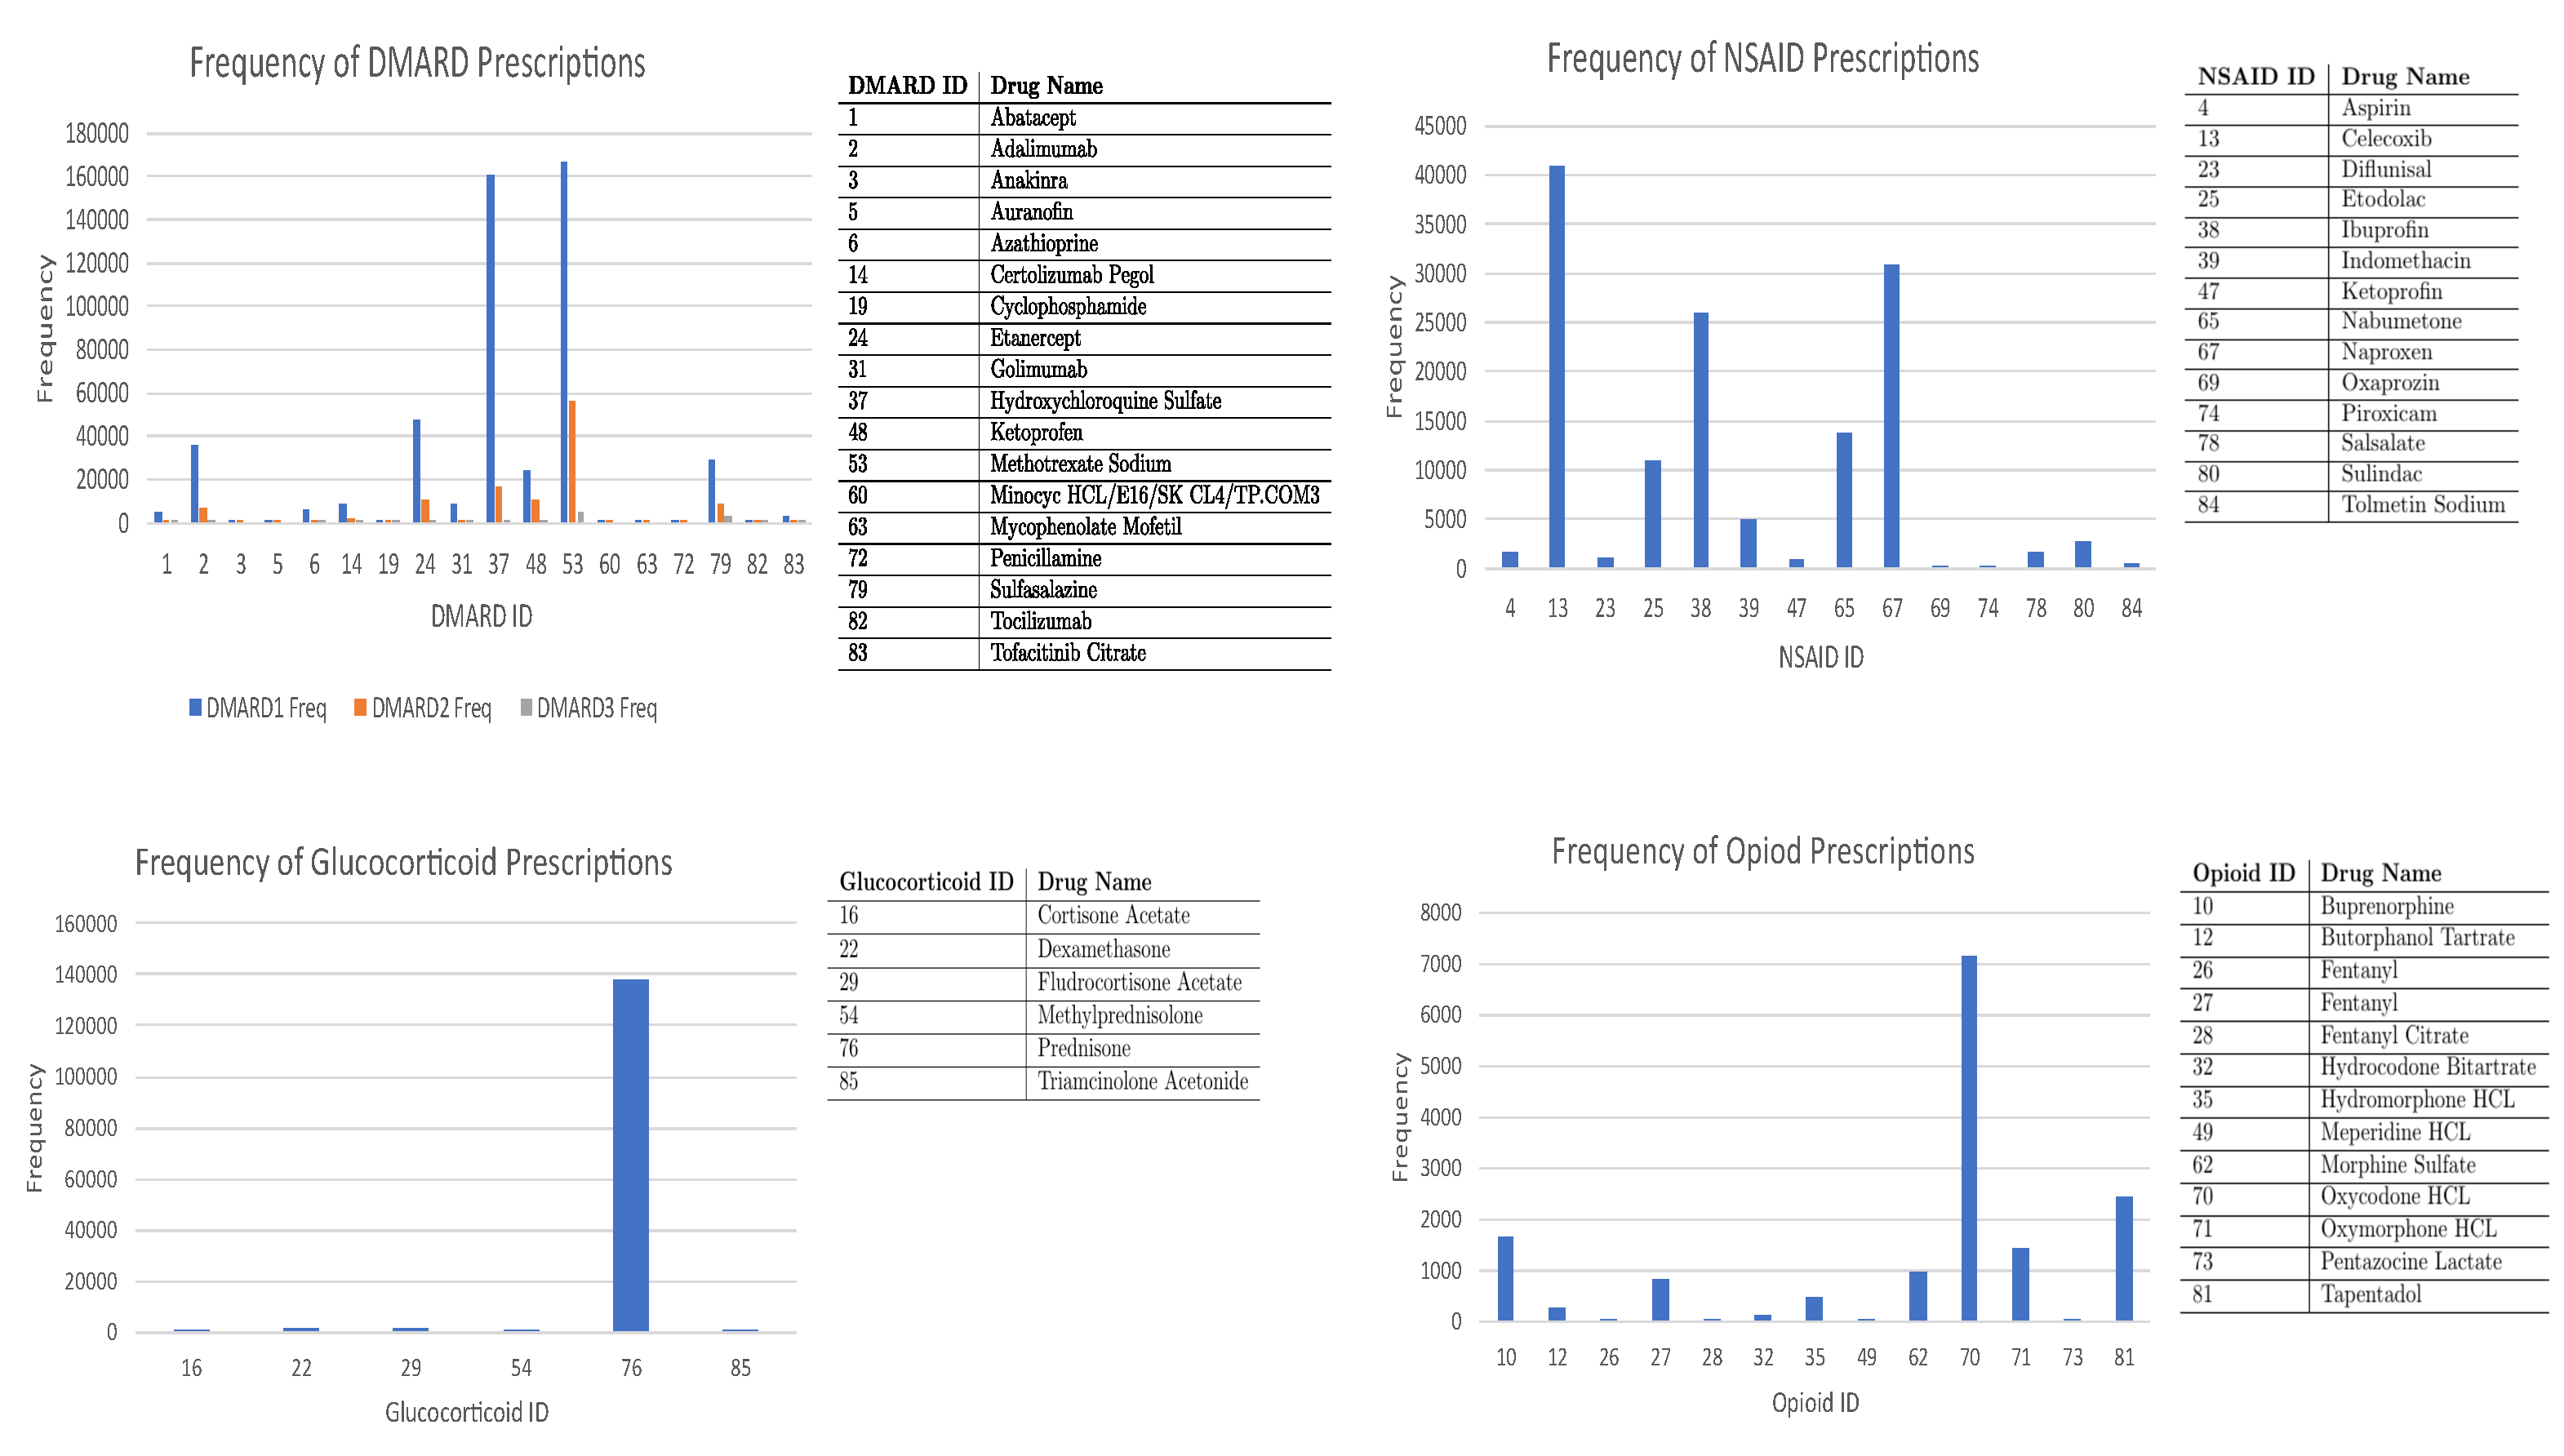
\includegraphics[width=.99\linewidth, scale=1.5]{Figures/TreatmentFrequency}
	\caption{This is a descriptive summary of the frequencies of medications prescribed to RA patients.}
	\label{fig:PrescriptionFrequency}
\end{figure}


To correlate a treatment with a patient, we examine the treatmentIDs. Each patient in this dataset have treatmentIDs that describe their treatment over time. They can be prescribed a DMARD, methotrexate (MTX), non tumor necrosis factor (nTNF), tumor necrosis factor (TNF) or tofacitinib (tofa). See Figure \ref{fig:ID} for an example of a patient's treatmentID.

\begin{figure}[H]
	\centering
	\includegraphics[width=.35\linewidth, scale=0.25]{Figures/TreatmentGroup}
	\caption{This is an example of a treatmentID. In this instance, the patient has been prescribed 1 DMARD and 1 TNF.}
	\label{fig:ID}
\end{figure}
	
DMARDs are used to slow down RA progression,and each of the categories in the treatmentID are DMARDS. The first category, labeled "DMARD", is any traditionally prescribed DMARD. MTX is a commonly used DMARD, and is also used to treat cancer patients. Both the DMARD and MTX categories are synthetic DMARDS. The nTNFs and TNFs are biologic DMARDs. nTNFs consist of monoclonal anti-TNF antibodies while TNFs contain soluble TNF receptors, and both of these methods inhibit NTF. Tofas are also biologic DMARDS, and work by inhibiting the JAK1 enzyme and disrupting cell signaling pathways. Because RA is a chronic illness, the patients treatments are dynamic and can change over time. Therefore, we also consider the frequency treatments change among all patient treatmentIDs. From Table \ref{changes}, we notice that most patients do not change their treatments over time. When they do, it is to stop taking a glucocorticoid or a painkiller.   


\begin{table}[H]
	\centering
	\begin{tabular}{l|l}
		\bf{Change In Treatment:} & \bf{Percentage} \\
		\hline
		No Glucocorticoid $\rightarrow$ Glucocorticoid & 4.17\% \\
		\hline
		Glucocorticoid $\rightarrow$ No Glucocorticoid & 17.84\% \\
		\hline
		No Painkiller $\rightarrow$ Painkiller &  3.54\% \\
		\hline
		Painkiller $\rightarrow$ No Painkiller & 9.08\% \\
		\hline
		Glucocorticoid $\rightarrow$ Painkiller & 1.18\% \\
		\hline
		Painkiller $\rightarrow$ glucocorticoid & 1.00\% \\
		\hline
		No Change & 63.18\% \\
		\hline
	\end{tabular}
	\caption{This table includes the average percent of treatment changes that occur over all treatmentID groups.}
	\label{changes}
\end{table}

The original dataset provided contained negative week values, indicating that the patient had been treated for RA prior to being diagnosed, determined by claims information. In Table \ref{negweeks}, we see that more patients receive treatment in the positive weeks than they do in the negative weeks. We also notice a higher instance of using both medications in the negative weeks. 

\begin{table}[H]
	\centering
	\begin{tabular}{l|l|l|l}
		~ & \textbf{Painkillers} & \textbf{Glucocorticoids} & \textbf{Both} \\
		\hline
		\textbf{- Weeks} & 37.2\% & 25.6\% & 18.0\% \\
		\hline
		\textbf{+ Weeks} & 47.1\% & 65.6\% & 15.7\% \\
		\hline
	\end{tabular}
	\caption{This table includes the percentage of medications prescribed to patients of the population of patients who received treatment.}
	\label{negweeks}
\end{table}

\hl{MISSING Pain Medications}\\

\hl{MISSING Treatment Changes} \\

\hl{MISSING frequency of treatments} \\

\begin{table}[H]
	\centering
	\begin{tabular}{l|l|l|l|l|l|l}
		~ & \textbf{IP Visits} & \textbf{IP Days} & \textbf{OP Visits} & \textbf{ER Visits} & \textbf{DR Visits} & \textbf{RX scripts} \\
		\hline
		\textbf{mean} & 0.0009 & 0.0037 & 0.1484 & 0.0039 & 0.3127 & 1.340 \\
		\hline
		\textbf{sd} & 0.0222 & 0.0836 & 0.3528 & 0.0492 & 0.5609 & 1.543 \\
		\hline
	\end{tabular}
	\caption{This table summarize the average and standard deviation over all treatmentIDs of medical visits and prescription fills.}
	\label{medVisits}
\end{table}

We also look at the average amount of times patients diagnosed with RA visited a medical facility or filled a prescription (RX script). In Table \ref{medVisits}, we account for medical visits including in patient (IP) visits, length of IP stay, out patient (OP) visits, emergency room (ER) visits, and doctor's (DR) visits. We find no statistical relevance of medical visits over the entire data set. This is due to the large amount of patients diagnosed with RA that did not seek treatment. 

Of the patients who received treatment, we observe how long patients waited to seek treatment after being diagnosed. To do this, we measure the time between the week the patient was diagnosed and the week when their treatment changed (TreatmentGroup = 1) by observing the WeekInd, a measure of weeks that passed since diagnosis. We can see in Figure \ref{fig:TreatmentHist} that the minimum duration is negative four weeks. The maximum duration is 336 weeks, almost six years. The average duration is around 28.72 weeks between diagnosis and treatment. We notice that this is a right-skew distribution, with most of the patients receiving treatment within the year they were diagnosed.

\begin{figure}[H]
	\centering
	%\captionsetup{justification=centering}
	\includegraphics[width=.55\linewidth, scale=.5]{Figures/TreatmentHist}
	\caption{This is a histogram of the time it took patients to begin treatment after being diagnosed.}
	\label{fig:TreatmentHist}
\end{figure}


\subsection{Data Cleaning}

Because treatment decisions are made on a monthly basis more often than on a weekly basis, we decide to collapse our data  from weekly intervals into monthly intervals. This change makes our data set more informative and less computationally expensive. To further simplify out dataset, we remove patients who never began treatment for RA over the entire course of the study. These patients are indicated by a treatment indicator, TreatmentIND, that is 0 if they receive no treatment and 1 if they receive treatment. To convert IP visits, IP days, OP visits, ER visits, DR visits, RX scripts into monthly intervals, we sum the occurrences over 4 weeks time. In addition, we create variables to tell us how many treatment changes occur in a given month, if a patient has taken a painkiller (0 if no, 1 if yes), if a person has taken a glucocorticoid (0 if no, 1 if yes), and assign each patient to a new treatment group (take the maximum number that occurs in each column in the treatmentID). The new treatment group contains five digits as the treatmentID does. 

After collapsing the data into monthly intervals, we remove thirty-eight patients with only one month of treatment data as we need a second month of data to determine the outcome during our analysis. Further data cleaning will be completed as needed in the analysis sections.       
        
\section{The Approach}
- Backward something something

- Identify the optimal dynamic treatment rules from observational data

\begin{equation}
(d^{opt}_1(X_1), d^{opt}_2(X_2) ... d^{opt}_n(X_n)) = \underset{a_1,a_2...a_n}{argmin} \mathds{E}\{Y|A_1=d_1(X_1), A_2=d_2(X_2)...A_n=d_n(X_n)\}
\end{equation}
Where:
\begin{table}[H]
	\centering
	\begin{tabular}{r l}
		$i =$ & $1,2,....n$ \\
		$d_i^{opt} \equiv$ & optimal decision at time point i \\
		$X_i \equiv$ & covariance at time point i \\
		$\mathds{E} \equiv $ & is the expected value \\
		$Y \equiv$ & outcome \\
		$A_i \equiv$ & treatment at time point i \\
		$d_i \equiv$ & decision at time point i \\	
	\end{tabular}
\end{table}
 
\begin{equation}
\mathds{E}(Y|A_1,X_1,A_2,X_2,...A_n,X_n) = f(A_1,X_1,A_2,X_2,...A_n,X_n)
\end{equation}
Where:
\begin{table}[H]
	\centering
	\begin{tabular}{r l}
		$f \equiv$ & a function fitted to the data set \\
	\end{tabular} 
\end{table}

\begin{equation}
\hat{d}_n(X_n, A_{n-11}, X_{n-1}...A_1,X_1) = \underset{a_n}{argmin}\hat{f}(A_1,X_1,A_2,X_2,...a_n,X_n) 
\end{equation}
Where:
\begin{table}[H]
	\centering
	\begin{tabular}{r l}
		$\hat{f} \equiv$ & is an estimated a function fitted to the data set \\
		$\hat{d}_n \equiv$ & is the estimated optimal decision at time point $i$ \\
		$i =$ & $1,2,....n$ \\
	\end{tabular} 
\end{table}


- Reduce the effects of confounding in observational studies \\

- in this case by observing the pseudo predicted value
\begin{equation}
Y^* = \underset{a_n}{min}\hat{f}(A_1,X_1,A_2,X_2,...a_n,X_n)
\end{equation}
Where:
\begin{table}[H]
	\centering
	\begin{tabular}{r l}
		$Y^* \equiv$ & predicted pseudo value \\
	\end{tabular} 
\end{table}

\begin{equation}
\mathds{E}(Y^*|A_i,X_i) = f(A_i,X_i)
\end{equation}

\begin{equation}
\hat{d_i}(X_i)= \underset{a_i}{argmin}f(a_i, X_i)
\end{equation}
%%%%%%%%%%%%%%%%%%%%%%%%%%%%%%%%%%%%%%%%%%%%%%%%%%%%%%%%%%%%%%%%%%%%%%%%%%%%%%%%%%%%%%%%%%%%%%%%%%%%%%
\subsection{A One Decision, Two Month Model} %cross-sectional data 
%%%%%%%%%%%%%%%%%%%%%%%%%%%%%%%%%%%%%%%%%%%%%%%%%%%%%%%%%%%%%%%%%%%%%%%%%%%%%%%%%%%%%%%%%%%%%%%%%%%%%%
- Condense the above to two months\\

- To get an idea if our defined outcome will work, and determine how it relates to the covariants

\begin{equation}
d^{opt}(X) = \underset{a\in domA}{argmin}\mathds{E} (Y|X=x, A=a)
\end{equation}

\begin{equation}
\mathds{E}(Y|X=x,A=a) = f(x,a)
\end{equation}

\begin{equation}
\hat{d}(x) = \underset{a\in A}{argmin}\hat{f}(x,a)
\end{equation}

- Measure of how well optimal rule works \\
 
- Also could be used as a prediction

\begin{equation}
\bar{Y} = \frac{1}{n}\sum_{i}^{n}Y_i
\end{equation}
Where 
\begin{table}[H]
	\centering
	\begin{tabular}{r l}
		$ \bar{Y} \equiv$ & average outcome \\
	\end{tabular} 
\end{table}

\begin{equation}
\tilde{Y} = \frac{\bigg(\sum_{i}^{n}\frac{Y_i\mathds{1}\{A_i=\hat{d}(x_i)\}}{\hat{P}(A_i|x_i)}\bigg)}{\bigg(\sum_{i}^{n}\frac{\mathds{1}\{A_i=\hat{d}(x_i)\}}{\hat{P}(A_i|x_i)}\bigg)}
\end{equation}
Where 
\begin{table}[H]
	\centering
	\begin{tabular}{r l}
		$ \tilde{Y} \equiv$ & estimation of the expectation\\
		$\hat{P} \equiv$ & propensity score\\
	\end{tabular} 
\end{table}

\subsubsection{Data Set}
We further clean the data for this section by eliminating uncommon treatmentIDs. We define uncommon treatmentIDs as an ID  less than 100 patients. The remaining TreatmentIDs for this section can be observed in Table \ref{ids1}. We remove these patients from this dataset for a couple reasons. The first is we want to avoid creating singular covariant matrices. The second is that we do not have enough replicates of these patients to make significant statistical conclusions regarding their TratmentIDs.

\begin{table}[H]
	\centering
	\begin{tabular}{c}
		\textbf{TreatmentID} \\
		\hline
		00010 \\
		01000 \\
		10000 \\
		11000 \\
	\end{tabular}
	\caption{Remaining TreatmentIDs after data cleaning.}
	\label{ids1}
\end{table}

\subsubsection{Model Selection}

To find a $\hat{f}(x,a)$ fit for our data set, we use to methods: Random forest and logistic regression. The random forest algorithm is implemented using the random forest package in R. The logistic regression algorithm is implemented using GLM in R. From these two methods, we examine the top five covariates and determine which covariates, $X$, to use in the approach.

\subsection{A Two Decision, Three Month Model}




\section{Computational Results}

\subsection{A One Decision, Two Month Model}

\subsection{A Two Decision, Three Month Model}


\section{Summary and Future Work}
\begin{itemize}
\item Briefly summarize your contributions, and their possible
impact on the field (but don't just repeat the abstract or introduction).
\item Identify the limitations of your approach.
\item Suggest improvements for future work.
\item Outline open problems.
\end{itemize}



\end{document}